\documentclass{beamer}

\mode<presentation> {
% Colors

%\usetheme{default}
%\usetheme{AnnArbor}
%\usetheme{Antibes}
%\usetheme{Bergen}
%\usetheme{Berkeley}
%\usetheme{Berlin}
%\usetheme{Boadilla}
%\usetheme{CambridgeUS}
%\usetheme{Copenhagen}
%\usetheme{Darmstadt}
%\usetheme{Dresden}
%\usetheme{Frankfurt}
%\usetheme{Goettingen}
%\usetheme{Hannover}
\usetheme{Ilmenau}
%\usetheme{JuanLesPins}
%\usetheme{Luebeck}
%\usetheme{Madrid}
%\usetheme{Malmoe}
%\usetheme{Marburg}
%\usetheme{Montpellier}
%\usetheme{PaloAlto}
%\usetheme{Pittsburgh}
%\usetheme{Rochester}
%\usetheme{Singapore}
%\usetheme{Szeged}
%\usetheme{Warsaw}

%Themes

%\usecolortheme{albatross}
%\usecolortheme{beaver}
%\usecolortheme{beetle}
%\usecolortheme{crane}
%\usecolortheme{dolphin}
%\usecolortheme{dove}
%\usecolortheme{fly}
%\usecolortheme{lily}
%\usecolortheme{orchid}
%\usecolortheme{rose}
%\usecolortheme{seagull}
%\usecolortheme{seahorse}
%\usecolortheme{whale}
%\usecolortheme{wolverine}

%\setbeamertemplate{footline} % To remove the footer line in all slides uncomment this line
%\setbeamertemplate{footline}[page number] % To replace the footer line in all slides with a simple slide count uncomment this line

\setbeamertemplate{navigation symbols}{} % To remove the navigation symbols from the bottom of all slides uncomment this line
}

\usepackage{graphicx} % Allows including images
\usepackage{booktabs} % Allows the use of \toprule, \midrule and \bottomrule in tables
\usepackage{tikz}
\usepackage{graphicx}
%----------------------------------------------------------------------------------------
%	TITLE PAGE
%----------------------------------------------------------------------------------------

\title[NMR Assignment with A*]{Accelerating Biomolecular Nuclear Magnetic Resonance Assignment with A*} % The short title appears at the bottom of every slide, the full title is only on the title page

\author[J. Venzke, P. Johnson, R. Davis, J. Emmons, K. Roth, D. Mascharka, L. Robison, T. Urness, A. Kilpatrick]{Joel Venzke, Paxten Johnson, Rachel Davis, John Emmons,\\ Katherine Roth, David Mascharka, Leah Robison,\\ Timothy Urness and Adina Kilpatrick} % Your name
\institute[Drake University] % Your institution as it will appear on the bottom of every slide, may be shorthand to save space
{
Department of Mathematics and Computer Science\\
Drake University\\

\medskip
\textit{joel.venzke@drake.edu} % Your email address
}
\date{April 10,2014} % Date, can be changed to a custom date

\begin{document}

\begin{frame}
\titlepage % Print the title page as the first slide
\end{frame}

% =======================================================================
% =======================================================================
\section{Introduction}
\begin{frame}
\frametitle{Overview} % Table of contents slide, comment this block out to remove it
\tableofcontents 
\end{frame}

\subsection{Motivation} 
\begin{frame}
	\frametitle{Motivation}
	\begin{itemize}
		\item Nuclear Magnetic Resonance Spectroscopy
		\begin{itemize}
			\item Gain knowledge about protein structure
			\item Study how mutations lead to diseases
		\end{itemize}
		\item Problems
		\begin{itemize}
			\item Generates large amounts of data
			\item Data analysis is slow and error prone 
		\end{itemize}
		\item Goal
		\begin{itemize}
			\item Automate the assignment process
			\item Decrease human error
			\item Increase productivity
		\end{itemize}
	\end{itemize}
\end{frame}

% =======================================================================
\subsection{Nuclear Magnetic Resonance Spectroscopy} 
\begin{frame}
	\frametitle{Nuclear Magnetic Resonance (NMR)}
	\begin{itemize}
		\item Used to obtain structural information 
		\begin{itemize}
			\item Chemical shift values
		\end{itemize}
		\item HNCACB experiment
		\begin{itemize}
			\item Generates $C_\alpha$ and $C_{\beta}$ residue $i$ and $i-1$
		\end{itemize}
		\item CBCA(CO) NH experiment 
		\begin{itemize}
			\item Generates $C_\alpha$ and $C_{\beta}$ for residue $i$
			\item Confirms residue data
		\end{itemize}
	\end{itemize}
\end{frame}

\begin{frame}
	\frametitle{Chemical Shift Values}
	\begin{figure}[H]
	\begin{center}
	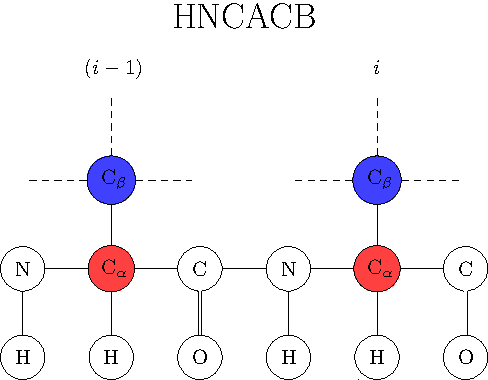
\includegraphics[width=.65\textwidth]{diagram}
	\end{center}
	\end{figure}
\end{frame}



% =======================================================================
% =======================================================================
\section{NMR Assignment Overview}

% =======================================================================
\subsection{Data Collection and Manual Assignment}
\begin{frame}
	\frametitle{Time Line}
	
	\vspace{1.5cm}
	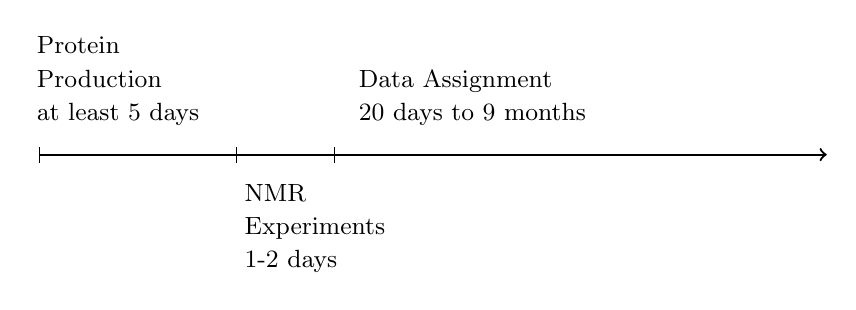
\begin{tikzpicture} [scale=.5]

		\draw [thick, ->] (0,0) -- (20,0);

		\draw (0,-.2) -- (0, .2);

		\draw (5,-.2) -- (5, .2);

		\draw (7.5,-.2) -- (7.5, .2);

		\node[align=left, above] at (2,.5)%
		{\small Protein\\ \small Production\\ \small at least 5 days};

		\node[align=left, below] at (7,-.5)%
		{\small NMR\\ \small Experiments\\ \small 1-2 days};

		\node[align=left, above] at (11,.5)%
		{\small Data Assignment\\ \small 20 days to 9 months};
	\end{tikzpicture}

	\vspace{1cm}
	\hfill \scriptsize\cite{babak_alipanahi_error_2011}
\end{frame}

\begin{frame}
	\frametitle{Manual Methods}
	\begin{itemize}
		\item Most time consuming part
		\item Prone to human error
		\item Missing and ambiguous data forces chunks to be skipped
	\end{itemize}

\end{frame}


% =======================================================================
% =======================================================================
\section{Automation Algorithm}

% =======================================================================
\subsection{Preprocessing}

\begin{frame}
	\frametitle{Initialization}
	\begin{itemize}
		\item Input
		\begin{itemize}
			\item Expected amino acid sequence
			\begin{itemize}
				\item Covered to expectation chemical shift values
				\item Stored as the protein chain
			\end{itemize}
			\item NMR chemical shift data
			\begin{itemize}
				\item $C_\alpha$ and $C_{\beta}$ for residue $i$ and $i-1$
				\item Stored in a tile
			\end{itemize}
		\end{itemize}
		\item Missing data
		\begin{itemize}
			\item Place holder tile generation
		\end{itemize}
		\item Grouping 
	\end{itemize}
\end{frame}

\begin{frame}
	\frametitle{Grouping}
	\begin{figure}[H]
	\begin{center}
	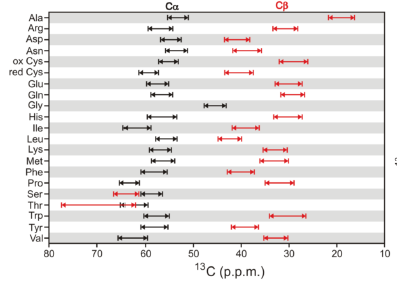
\includegraphics[width=.65\textwidth]{carbon}
	\end{center}
	\end{figure}
\hfill \scriptsize\cite{carbon}
\end{frame}

% =======================================================================
\subsection{Assignment}

\begin{frame}
	\frametitle{Starting the assignment}
	\begin{tikzpicture} [scale=.5]
		\draw [thick] (1.5,6.5) -- (13.5,6.5) -- (13.5,3.5) -- (1.5,3.5) -- (1.5,6.5);
		\node[align=center] at (4.5,5) {\textbf{Tiles to assign:}};
		\node[align=center, box, draw] at (8.5,5) {13\\9};
		\node[align=center, box, draw] at (10.5,5) {11\\13};
		\node[align=center, box, draw] at (12.5,5) {9\\12};		
		\draw [thick] (-4,2) -- (18,2);

		\node[align=right] at (11,2.5) {\textbf{Tiles}};

		\node[align=center, box, draw, fill = green] at (5,0) {13\\9};
		\node[align=center] at (6.5,0) {1.5};
		\node[align=center, box, draw, fill = green] at (11,0) {11\\13};
		\node[align=center] at (12.5,0) {0.5};
		\node[align=center, box, draw, fill = green] at (16.5,0) {9\\12};
		\node[align=center] at (18,0) {2.5};


		\draw [thick] (2,3) -- (2,-6);

		\node[align=right] at (-1,2.5) {\textbf{Protein Chain}};
		\node[align=right] at (-1,0) {11.5};
		\node[align=right] at (-1,-2.5) {12.5};
		\node[align=right] at (-1,-5) {9.6};

	\end{tikzpicture}
\end{frame}

\begin{frame}
	\frametitle{Cost Calculation}
	\begin{itemize}
		\item Accuracy matching the protein chain residue
		\item Accuracy matching the tile above current tile
		\item Cost of all tiles place before current tile
	\end{itemize}
\end{frame}

\begin{frame}
	\frametitle{Generating child nodes}
	\begin{tikzpicture} [scale=.5]
		\draw [thick] (1.5,6.5) -- (13.5,6.5) -- (13.5,3.5) -- (1.5,3.5) -- (1.5,6.5);
		\node[align=center] at (4.5,5) {\textbf{Tiles to assign:}};
		\node[align=center, box, draw] at (8.5,5) {13\\9};
		\node[align=center, box, draw] at (10.5,5) {11\\13};
		\node[align=center, box, draw] at (12.5,5) {9\\12};		
		\draw [thick] (-4,2) -- (18,2);

		\node[align=right] at (11,2.5) {\textbf{Tiles}};

		\node[align=center, box, draw, fill = orange] at (5,0) {13\\9};
		\node[align=center] at (6.5,0) {1.5};
		\node[align=center, box, draw, fill = orange] at (11,0) {11\\13};
		\node[align=center] at (12.5,0) {0.5};
		\node[align=center, box, draw, fill = orange] at (16.5,0) {9\\12};
		\node[align=center] at (18,0) {2.5};


		\draw [thick] (2,3) -- (2,-6);

		\node[align=right] at (-1,2.5) {\textbf{Protein Chain}};
		\node[align=right] at (-1,0) {11.5};
		\node[align=right] at (-1,-2.5) {12.5};
		\node[align=right] at (-1,-5) {9.6};

	\end{tikzpicture}
\end{frame}

\begin{frame}
	\frametitle{Generating child nodes}
	\begin{tikzpicture} [scale=.5]
		\draw [thick] (1.5,6.5) -- (13.5,6.5) -- (13.5,3.5) -- (1.5,3.5) -- (1.5,6.5);
		\node[align=center] at (4.5,5) {\textbf{Tiles to assign:}};
		\node[align=center, box, draw] at (8.5,5) {13\\9};
		\node[align=center, box, draw] at (10.5,5) {11\\13};
		\node[align=center, box, draw] at (12.5,5) {9\\12};		
		\draw [thick] (-4,2) -- (18,2);

		\node[align=right] at (11,2.5) {\textbf{Tiles}};

		\draw [thick, ->] (11,1.5) -- (11,1);
		\node[align=center, box, draw, fill = orange] at (5,0) {13\\9};
		\node[align=center] at (6.5,0) {1.5};
		\node[align=center, box, draw, fill = green] at (11,0) {11\\13};
		\node[align=center] at (12.5,0) {0.5};
		\node[align=center, box, draw, fill = orange] at (16.5,0) {9\\12};
		\node[align=center] at (18,0) {2.5};

		\draw (11,-1) -- (9.5,-1.5);
		\draw (11,-1) -- (13,-1.5);

		
		\node[align=center, box, draw, fill = orange] at (9.5,-2.5) {13\\9};
		\node[align=center] at (11,-2.5) {1.0};
		\node[align=center, box, draw, fill = orange] at (12.5,-2.5) {9\\12};
		\node[align=center] at (14,-2.5) {8.0};


		\draw [thick] (2,3) -- (2,-6);

		\node[align=right] at (-1,2.5) {\textbf{Protein Chain}};
		\node[align=right] at (-1,0) {11.5};
		\node[align=right] at (-1,-2.5) {12.5};
		\node[align=right] at (-1,-5) {9.6};

	\end{tikzpicture}
\end{frame}


\subsection{Goal State}
\begin{frame}
	\frametitle{Goal State}
	\begin{tikzpicture} [scale=.5]
		\draw [thick] (1.5,6.5) -- (13.5,6.5) -- (13.5,3.5) -- (1.5,3.5) -- (1.5,6.5);
		\node[align=center] at (4.5,5) {\textbf{Tiles to assign:}};
		\node[align=center, box, draw] at (8.5,5) {13\\9};
		\node[align=center, box, draw] at (10.5,5) {11\\13};
		\node[align=center, box, draw] at (12.5,5) {9\\12};		
		\draw [thick] (-4,2) -- (18,2);

		\node[align=right] at (11,2.5) {\textbf{Tiles}};

		\node[align=center, box, draw, fill = orange] at (5,0) {13\\9};
		\node[align=center] at (6.5,0) {1.5};
		\node[align=center, box, draw, ] at (11,0) {11\\13};
		\node[align=center] at (12.5,0) {0.5};
		\node[align=center, box, draw, fill = orange] at (16.5,0) {9\\12};
		\node[align=center] at (18,0) {2.5};

		\draw (11,-1) -- (9.5,-1.5);
		\draw (11,-1) -- (13,-1.5);

		\draw [thick, ->] (9.5,-1) -- (9.5,-1.5);
		\node[align=center, box, draw, fill = green] at (9.5,-2.5) {13\\9};
		\node[align=center] at (11,-2.5) {1.0};
		\node[align=center, box, draw, fill = orange] at (12.5,-2.5) {9\\12};
		\node[align=center] at (14,-2.5) {8.0};

		\draw (9.5,-4) -- (9.5,-3.5);

		\node[align=center, box, draw, fill = orange] at (9.5,-5) {9\\12};
		\node[align=center] at (11,-5) {1.6};

		\draw [thick] (2,3) -- (2,-6);

		\node[align=right] at (-1,2.5) {\textbf{Protein Chain}};
		\node[align=right] at (-1,0) {11.5};
		\node[align=right] at (-1,-2.5) {12.5};
		\node[align=right] at (-1,-5) {9.6};

	\end{tikzpicture}
\end{frame}


\begin{frame}
	\frametitle{Goal State}
	\begin{tikzpicture} [scale=.5]
		\draw [thick] (1.5,6.5) -- (13.5,6.5) -- (13.5,3.5) -- (1.5,3.5) -- (1.5,6.5);
		\node[align=center] at (4.5,5) {\textbf{Tiles to assign:}};
		\node[align=center, box, draw] at (8.5,5) {13\\9};
		\node[align=center, box, draw] at (10.5,5) {11\\13};
		\node[align=center, box, draw] at (12.5,5) {9\\12};		
		\draw [thick] (-4,2) -- (18,2);

		\node[align=right] at (11,2.5) {\textbf{Tiles}};

		\draw [thick, ->] (5,1.5) -- (5,1);
		\node[align=center, box, draw, fill = green] at (5,0) {13\\9};
		\node[align=center] at (6.5,0) {1.5};
		\node[align=center, box, draw] at (11,0) {11\\13};
		\node[align=center] at (12.5,0) {0.5};
		\node[align=center, box, draw, fill = orange] at (16.5,0) {9\\12};
		\node[align=center] at (18,0) {2.5};

		\draw (11,-1) -- (9.5,-1.5);
		\draw (11,-1) -- (13,-1.5);

		\node[align=center, box, draw] at (9.5,-2.5) {13\\9};
		\node[align=center] at (11,-2.5) {1.0};
		\node[align=center, box, draw, fill = orange] at (12.5,-2.5) {9\\12};
		\node[align=center] at (14,-2.5) {8.0};


		\draw (5,-1) -- (3.5,-1.5);
		\draw (5,-1) -- (6.5,-1.5);

		\node[align=center, box, draw, fill = orange] at (3.5,-2.5) {13\\9};
		\node[align=center] at (5,-2.5) {6.0};
		\node[align=center, box, draw, fill = orange] at (6.5,-2.5) {9\\12};
		\node[align=center] at (8,-2.5) {5.0};

		\draw (9.5,-4) -- (9.5,-3.5);

		\node[align=center, box, draw, fill = orange] at (9.5,-5) {9\\12};
		\node[align=center] at (11,-5) {1.6};

		\draw [thick] (2,3) -- (2,-6);

		\node[align=right] at (-1,2.5) {\textbf{Protein Chain}};
		\node[align=right] at (-1,0) {11.5};
		\node[align=right] at (-1,-2.5) {12.5};
		\node[align=right] at (-1,-5) {9.6};

	\end{tikzpicture}
\end{frame}

\begin{frame}
	\frametitle{Solution State}
	\begin{tikzpicture} [scale=.5]
		\draw [thick] (1.5,6.5) -- (13.5,6.5) -- (13.5,3.5) -- (1.5,3.5) -- (1.5,6.5);
		\node[align=center] at (4.5,5) {\textbf{Tiles to assign:}};
		\node[align=center, box, draw] at (8.5,5) {13\\9};
		\node[align=center, box, draw] at (10.5,5) {11\\13};
		\node[align=center, box, draw] at (12.5,5) {9\\12};		
		\draw [thick] (-4,2) -- (18,2);

		\node[align=right] at (11,2.5) {\textbf{Tiles}};

		\node[align=center, box, draw] at (5,0) {13\\9};
		\node[align=center] at (6.5,0) {1.5};
		\node[align=center, box, draw, fill = green] at (11,0) {11\\13};
		\node[align=center] at (12.5,0) {0.5};
		\node[align=center, box, draw, fill = orange] at (16.5,0) {9\\12};
		\node[align=center] at (18,0) {2.5};

		\draw (11,-1) -- (9.5,-1.5);
		\draw (11,-1) -- (13,-1.5);

		\node[align=center, box, draw, fill = green] at (9.5,-2.5) {13\\9};
		\node[align=center] at (11,-2.5) {1.0};
		\node[align=center, box, draw, fill = orange] at (12.5,-2.5) {9\\12};
		\node[align=center] at (14,-2.5) {8.0};


		\draw (5,-1) -- (3.5,-1.5);
		\draw (5,-1) -- (6.5,-1.5);

		\node[align=center, box, draw, fill = orange] at (3.5,-2.5) {13\\9};
		\node[align=center] at (5,-2.5) {6.0};
		\node[align=center, box, draw, fill = orange] at (6.5,-2.5) {9\\12};
		\node[align=center] at (8,-2.5) {5.0};

		\draw (9.5,-4) -- (9.5,-3.5);

		\node[align=center, box, draw, fill = green] at (9.5,-5) {9\\12};
		\node[align=center] at (11,-5) {1.6};

		\draw [thick] (2,3) -- (2,-6);

		\node[align=right] at (-1,2.5) {\textbf{Protein Chain}};
		\node[align=right] at (-1,0) {11.5};
		\node[align=right] at (-1,-2.5) {12.5};
		\node[align=right] at (-1,-5) {9.6};

	\end{tikzpicture}
\end{frame}

% =======================================================================
% =======================================================================
\section{Conclusion}

% =======================================================================
\subsection{Results}

\begin{frame}
	\frametitle{Time of Assignment}
	\begin{figure}[H]
	\begin{center}
	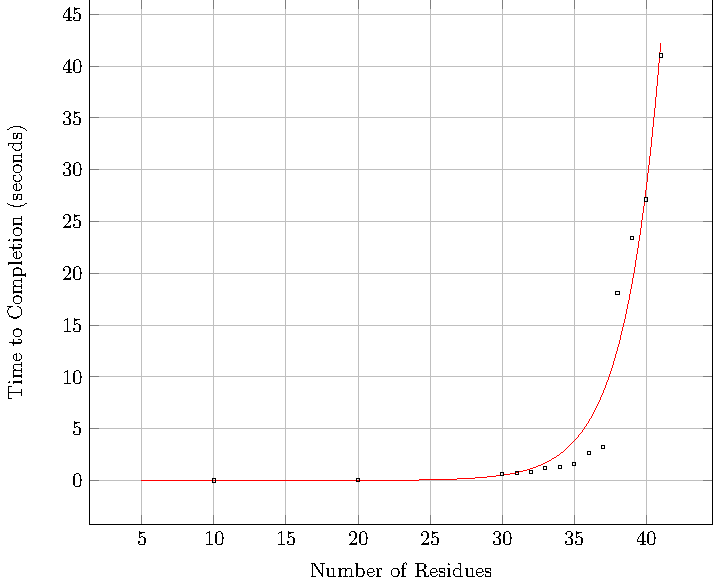
\includegraphics[width=.65\textwidth]{plot}
	\end{center}
	\end{figure}
\end{frame}


% =======================================================================
\subsection{Outlook}
\begin{frame}
	\frametitle{Future Goals}
	\begin{itemize}
		\item Parallelization
		\begin{itemize}
			\item Decrease assignment time
			\item Allow for larger data sets
		\end{itemize}
		\item Machine learning 
		\begin{itemize}
			\item Increase accuracy of assignment
			\item Optimize cost calculation
		\end{itemize}
	\end{itemize}
\end{frame}

\begin{frame}
	\frametitle{Acknowledgments}
	\begin{itemize}
		\item Dr. Tim Urness (Mathematics and Computer Science)
		\item Dr. Adina Kilpatrick (Physic)
		\item Rachel Davis (research colleague)
		\item John Emmons (research colleague)
		\item  Katherine Roth (research colleague)
		\item  David Mascharka (research colleague)
		\item  Leah Robison (research colleague)
	\end{itemize}
\end{frame}

\begin{frame}{Bibliography}
\bibliographystyle{amc}
\bibliography{presentaion}
\end{frame}

\begin{frame}
	\frametitle{Thank You} 
	\begin{center}
	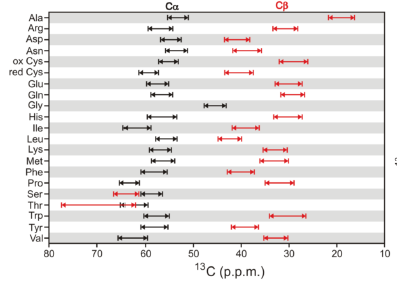
\includegraphics[width=0.3\textwidth]{carbon}\hspace{2em}
	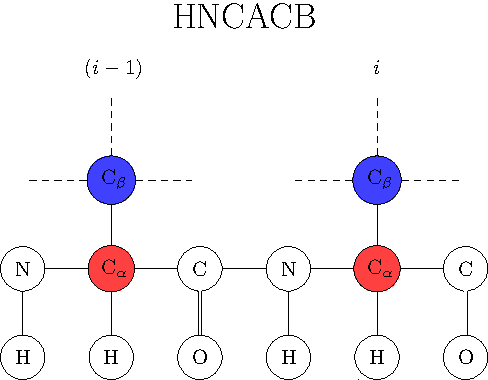
\includegraphics[width=0.3\textwidth]{diagram}
	\end{center}
	\begin{center}
	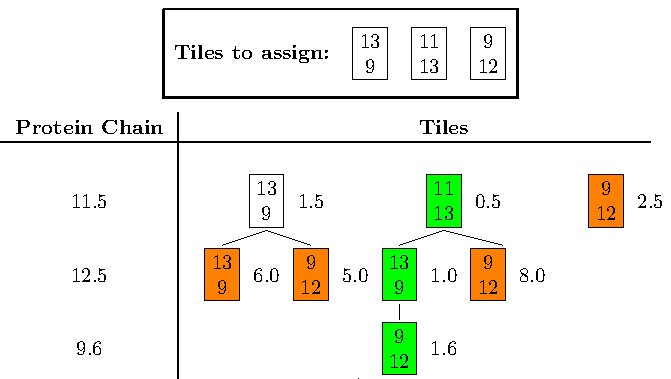
\includegraphics[width=0.4\textwidth]{time_line}\hspace{2em}
	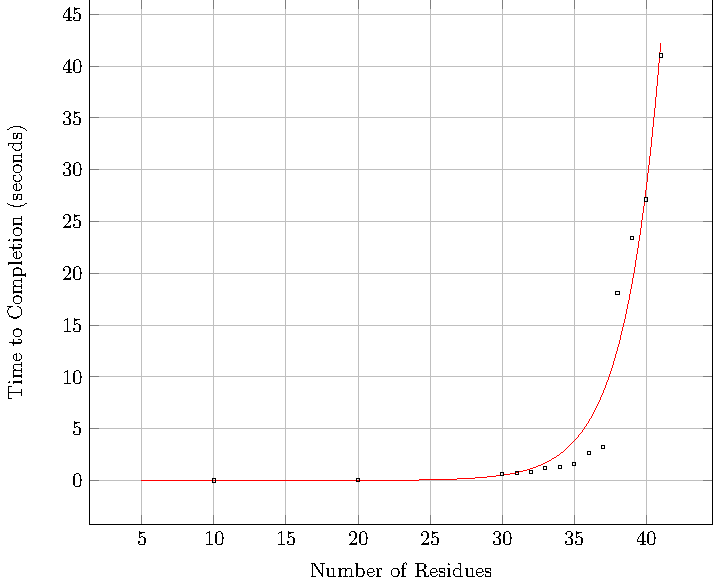
\includegraphics[width=0.3\textwidth]{plot}
\end{center}
\end{frame}

\end{document}